\chapter{Dark matter overview}\label{chap:DarkMatterOverview}
\section{Evidence for dark matter}\label{sec:DMOverview/Evidence4DM}
In the latter part of the 19th century, astronomers began to propose the existence of non-luminous matter to account for the uneven distribution of stars observed in the night sky \cite{HistoryofDM}. One of the earliest quantitative attempts to estimate the presence of such "dark bodies" in the Milky Way was made by Lord Kelvin in 1904. Kelvin postulated that if stars in the Milky Way could be modelled analogously to particles in a gas, interacting primarily through gravity, then a relationship could be established between the size of the system and the velocity dispersion of its constituents \cite{Kelvin1904}. The term \textit{dark matter} (\textit{mati\`ere obscure}) was first introduced by Henri Poincar\`e in 1906. Based on Kelvin’s velocity dispersion calculations, Poincar\`e argued that the amount of dark matter was likely to be less than or equal to the amount of visible matter \cite{HPon}. In 1922, Jacobus Kapteyn developed one of the earliest models to quantitatively describe the size and structure of the Milky Way. His model characterized the stellar distribution as a flattened disk rotating about an axis aligned with the galactic pole. Kapteyn reached conclusions similar to those of Poincaré, asserting that the presence of significant quantities of unseen matter was improbable \cite{Kapteyn1922}.

While these early investigations did not yield definitive evidence for the existence of dark matter, they established a foundational framework upon which later studies would build more rigorous arguments for the presence of missing mass in the Galaxy.

\subsection{Virial theorem and the Coma Cluster}\label{sec:DMOverview/ViralTheorem}
The virial theorem is a fundamental result in classical mechanics that relates the average total kinetic energy $\langle T \rangle$ of a system to its average total potential energy $\langle U \rangle$. The theorem can be used to estimate the mass of a galaxy cluster through the following approximation:
\begin{equation}
\begin{split}
2\langle T \rangle + \langle U \rangle = 0, \\
Nm\langle v^2\rangle - \frac{3}{5}\frac{GN^2m^2}{R}=0,\\
Nm=\frac{5R\langle v_r^2 \rangle}{G},\\
\end{split}
\label{eq:DMOverview/virial}
\end{equation}
where $N$ is the estimate number of galaxies in the cluster, $M$ is the observed seller mass of the galaxies in the cluster, $v_r$ is the radial velocities, and $R$ is the radius of the cluster.
In 1933, Fritz Zwicky applied the virial theorem to the Coma Cluster of galaxies \cite{Zwicky1933}. He measured the radial velocities of galaxies within the cluster and estimated their velocity dispersion. When he used the virial theorem to estimate the total mass required to gravitationally bind the system, he estimated the minimum mass of the galaxies in the cluster to be $M=4\times 10^{10}M_{\odot}$, where $M_{\odot}$ is one solar mass. With an average velocity dispersion observed to be approximately 1000~kms$^{-1}$, the mass-to-light ratio that was far too large to be accounted for by visible matter alone \cite{HistoryofDM}. Zwicky’s analysis revealed that the total mass inferred from the virial theorem was roughly 400 times greater than what could be explained by the luminous matter. To resolve this discrepancy, he proposed the existence of a substantial amount of unseen mass, which he referred to as \textit{dunkle Materie}, or “dark matter” \cite{Zwicky1933}.

\subsection{Galaxy rotation curves}\label{sec:DMOverview/RotationCurves}
A galaxy rotation curve describes the variation of orbital velocity of stars and gas as a function of their radial distance from the galactic centre. Under the assumption that a galaxy's mass is distributed entirely within its luminous matter, one would expect the mass to be concentrated primarily near the galactic centre. Therefore, the orbital velocity of objects situated at large radii should decrease with distance, according a Keplerian dynamics given by:
\begin{equation}
v(r) \propto \frac{1}{\sqrt{r}},
\end{equation}
where $v(r)$ is the orbital velocity and $r$ is the radial distance from the galactic centre.
In 1978, Vera C. Rubin \textit{et al.}\cite{Rubin} analysed the hydrogen spectra from a sample of ten high-luminosity spiral galaxies. By measuring the Doppler shift of the 21~cm line in the hydrogen spectra, they were able to determine the rotation velocities of gas and stars across a range of galactic radii. Rubin found that the rotation curves of these galaxies remained approximately constant, whilst the orbital velocities stayed constant, even at large radii. This observation was inconsistent with the mass inferred from visible matter alone and the expectations resulting from applied Keplerian dynamics.
A representative velocity profile for the galaxy NGC 6503 is shown in \autoref{fig:NGC6503}. The high orbital velocities at large radii suggests that a significant portion of galactic mass must be distributed well beyond the visible edge. This led to the hypothesis of a surrounding, non-luminous mass component, commonly referred to as a dark matter ``halo'' that provides the additional gravitational influence required to maintain the observed rotation velocities. The presence of such halo could explain the observed phenomena.
\begin{figure}[ht]
	\centering
	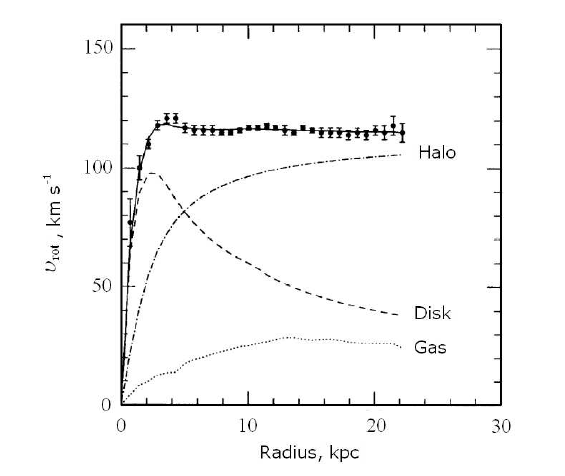
\includegraphics[width = 0.6\textwidth]{figures/DMOverview/NGC_6503.png}
	\caption[Galactic rotation curve for NGC 6503.]{Galactic rotation curve for NGC 6503. The dotted and dashed lines represents where the data should lie if Keplerian dynamics are obeyed. The dot-dashed line indicates the dark matter `halo' contribution needed for the function to fit the data \cite{Freese2009}.}
	\label{fig:NGC6503}
\end{figure}
\subsection{Gravitational lensing}\label{sec:DMOverview/GravLens}
The observed effect of gravitational lensing can be used to infer the total mass of astronomical objects. An example of the effect gravitational lensing has on light from a distant galaxy is shown in \autoref{fig:DMOverview/GravLens}. The effect was first described theoretically by Albert Einstein in 1936 \cite{GravLens}. The effect occurs when a massive object (lensing object) is situated in the line of sight between a distant source and an observer. Due to the gravitational field of the lensing object, light from the source deflects from its path resulting in observable distortions such as magnification, image splitting, or the formation of arcs and rings.
When the lensing is strong enough to produce multiple images or highly distorted arcs, it is referred to as \textit{strong gravitational lensing}. An example of such an effect is shown in \autoref{fig:DMOverview/StrongGravLens}. The degree of light deflection depends on the gravitational potential of the lensing object, which can be reconstructed by analysing the extent and geometry of the observed distortions \cite{Young2016}.

The mass of the lensing object in the line of sight is compared with that of the observed baryonic matter (stars, dust and gas), and the existence of dark matter is inferred to explain the discrepancy between the visible mass and lensing mass. 
\begin{figure}[ht!]
	\centering
	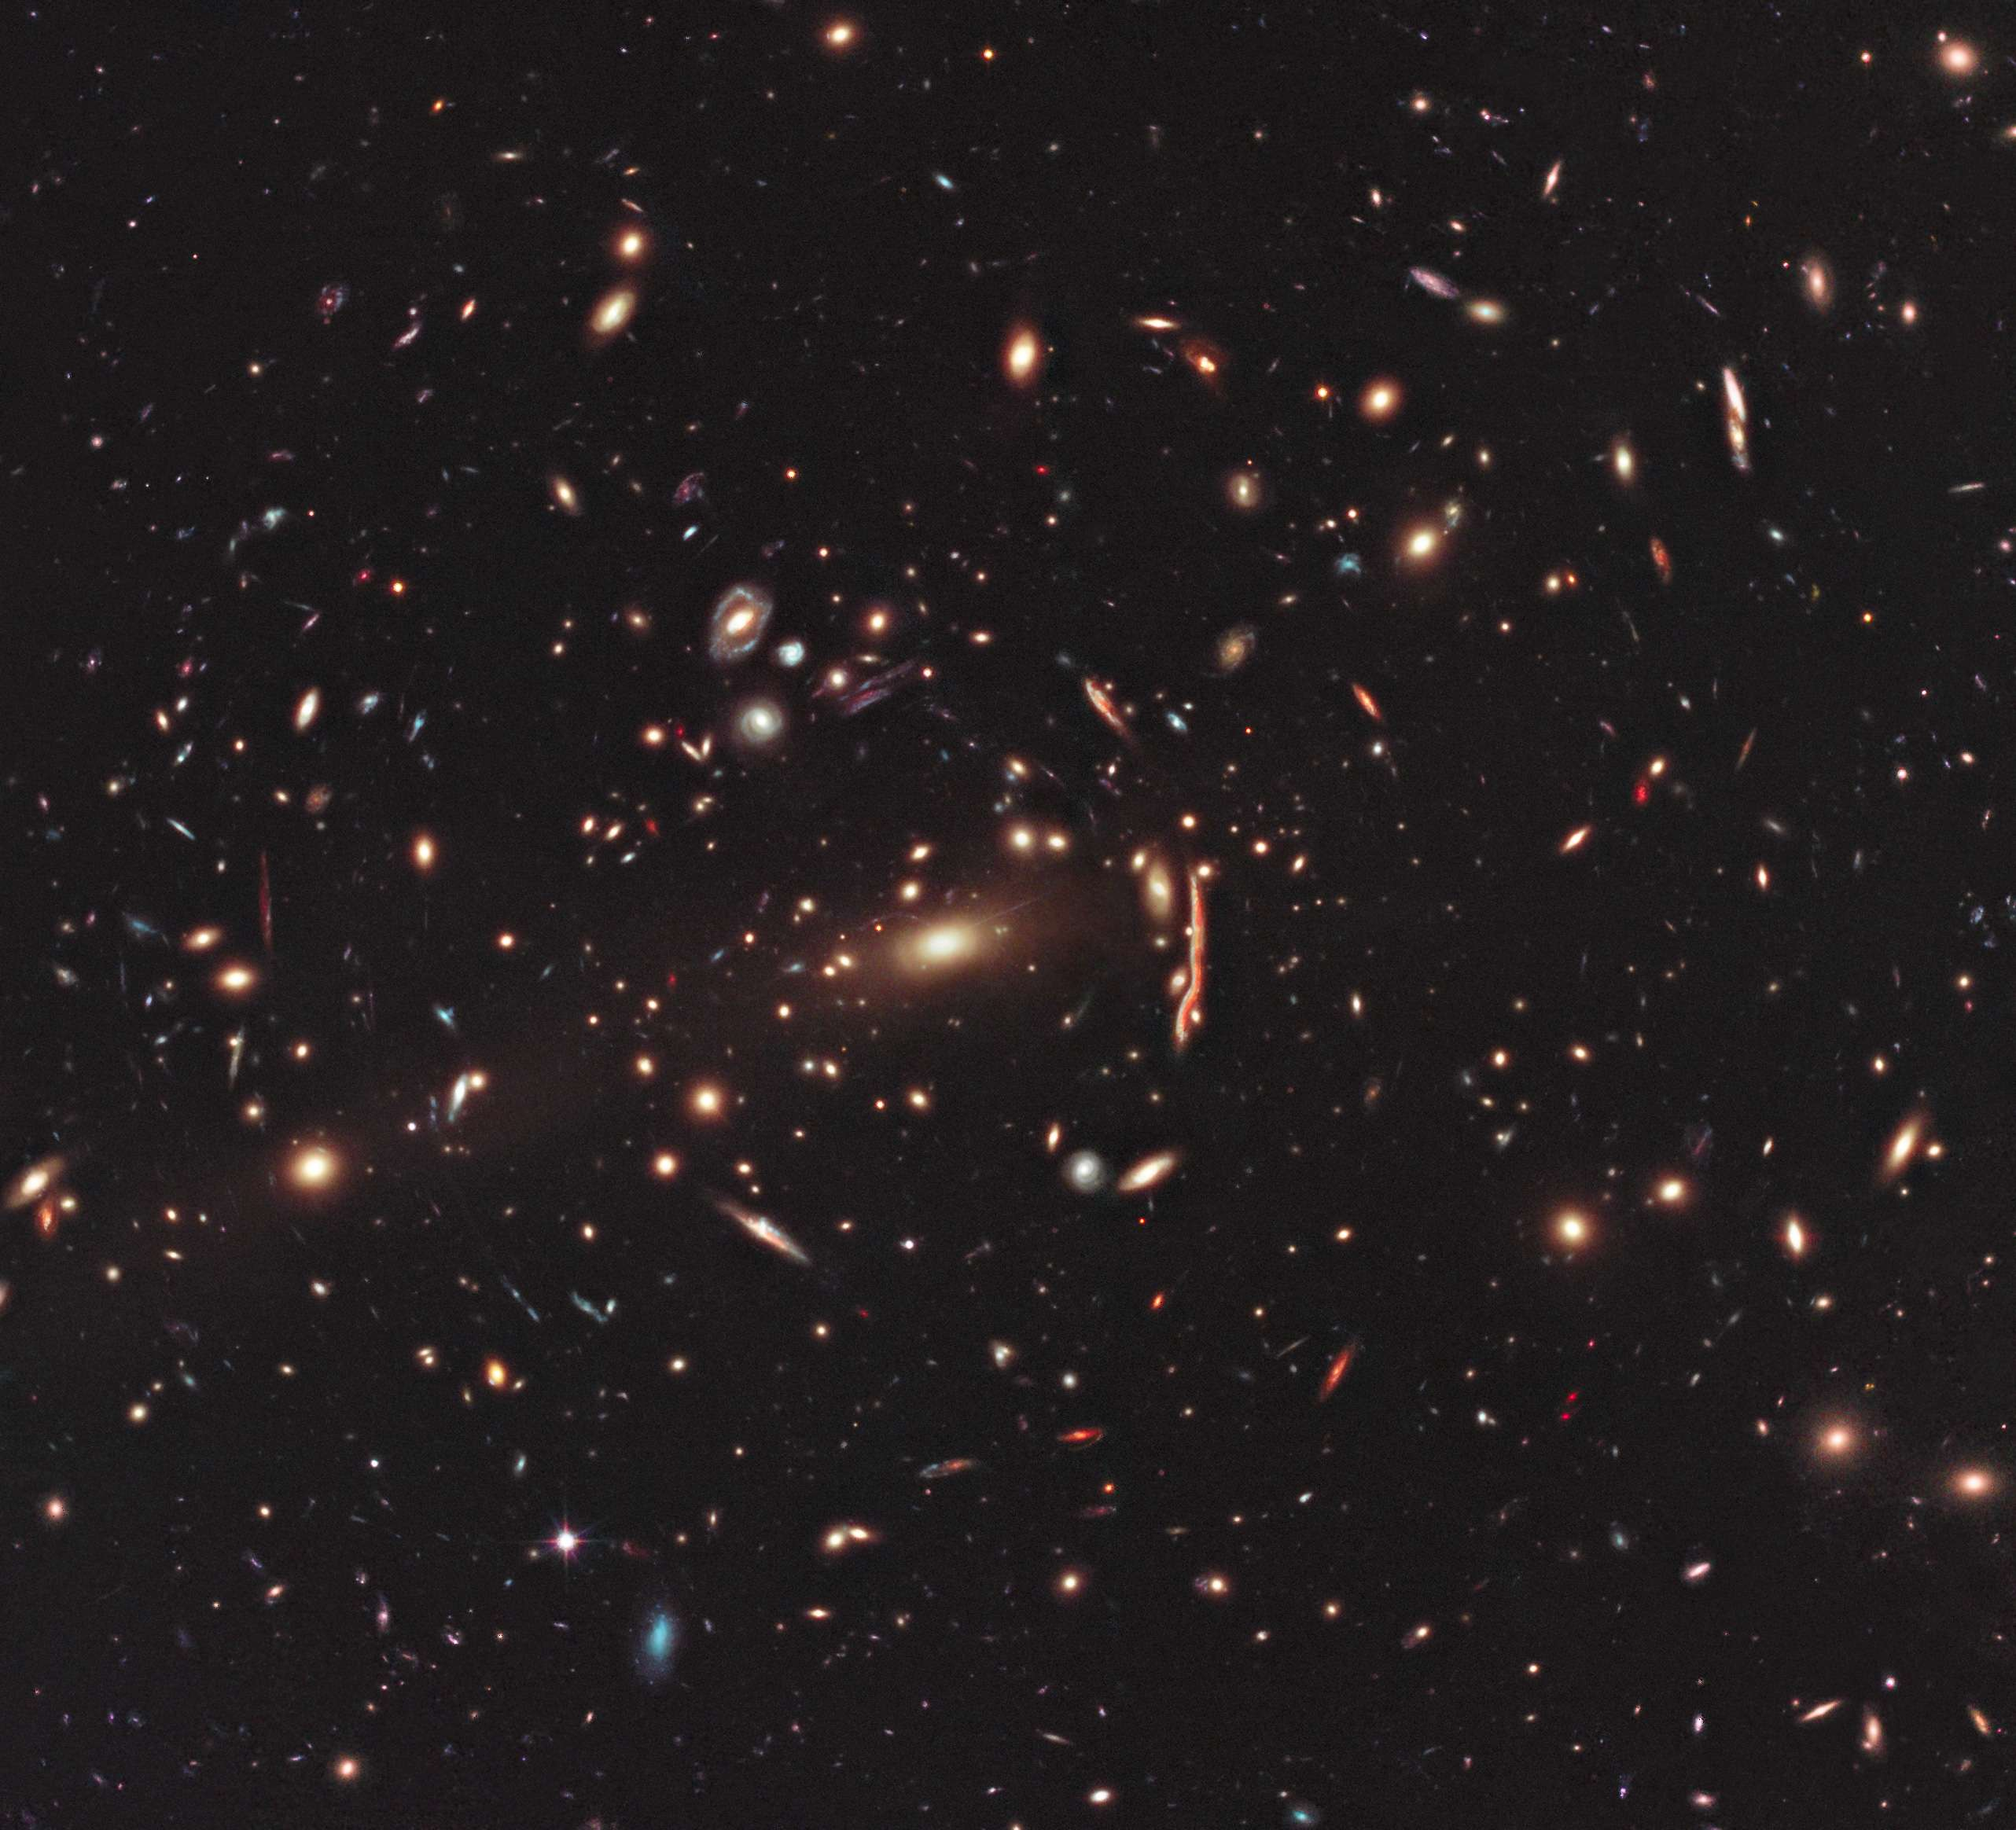
\includegraphics[width=0.7\textwidth]{figures/DMOverview/GravLensIm.jpg}
	\caption[Gravitational lensing by the galaxy cluster MACS J1206.2-0842s.]{Gravitational lensing by the galaxy cluster MACS J1206.2-0842s \cite{GravLensPicture}. The image was taken by the NASA/ESA Hubble Space Telescope, this galaxy is one of 25 clusters being studied as part of the Cluster Lensing and Supernova survey with Hubble programme.}
	\label{fig:DMOverview/GravLens}
\end{figure}

\begin{figure}[ht!]
	\centering
	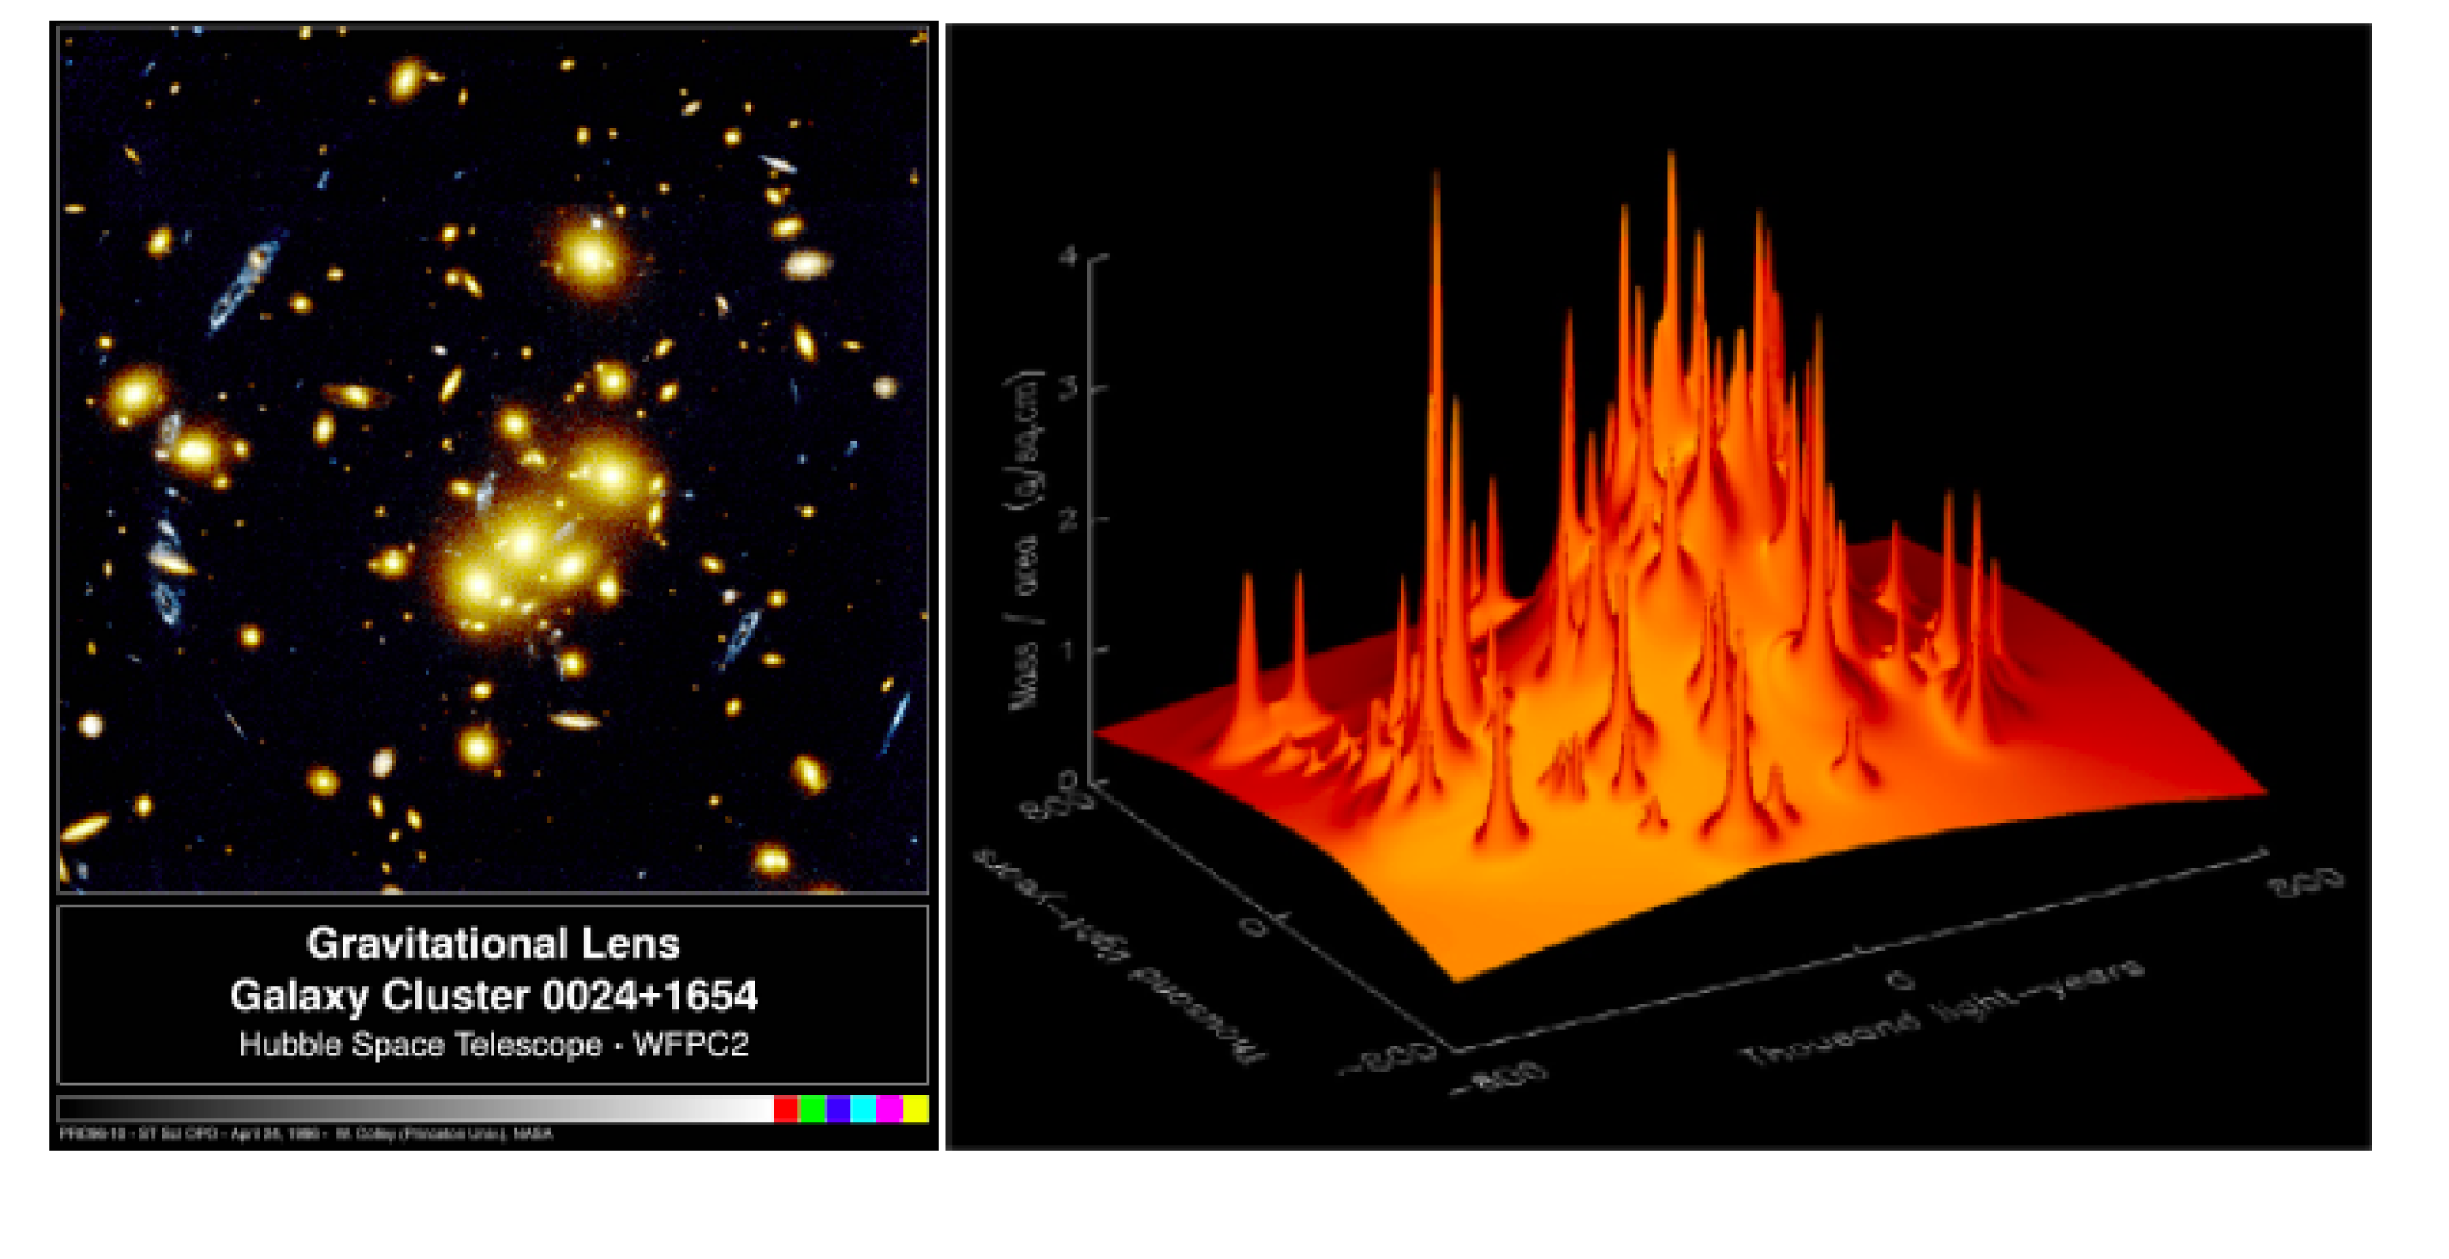
\includegraphics[width=0.8\textwidth]{figures/DMOverview/Strong_Grav_lens.png}
	\caption[\textbf{Left:} Effects of gravitational lensing on multiple galaxies. \textbf{Right:} Reconstruction of gravitational lensing effects.]{\textbf{Left:} An image from the Hubble Space Telescope where the foreground cluster of galaxies gravitationally lenses the blue background galaxy. \textbf{Right:} A reconstruction of gravitational lensing by galaxy cluster. Baryonic matter within the cluster are represented by the sharp spikes and the smooth background component corresponds to some non-visible mass \cite{Freese2009}.}
	\label{fig:DMOverview/StrongGravLens}
\end{figure}
\subsubsection{The Bullet Cluster}\label{sec:DMOverview/BulletCluster}
Observations of the Bullet Cluster (1E 0657–56) made by the Hubble Space Telescope and the Chandra X-ray Observatory provides evidence towards the existence of dark matter using gravitational lensing.
The Bullet Cluster consists of two galaxy clusters which have collided and are now moving apart. A composite image of the cluster can be seen in \autoref{fig:DMOverview/BulletComp}, where colour overlays represent the distribution of both luminous and total mass components. The blue regions in the image highlight the total mass distribution derived from gravitational lensing measurements, while the pink regions represent the hot, X-ray-emitting gas that contains the majority of the baryonic matter, such as gas and dust. Analysis of the X-ray data found that as the two clusters passed through one another, their gaseous components interacted strongly, colliding, slowing down, and heating up, thus producing intense X-ray emissions. Whereas measurements made using gravitational lensing indicated that the majority of the non-luminous portion of mass continued without disruption. The lensing mass peaks of the colliding clusters were compared with the X-ray peaks and an offset was found \cite{Clowe_2004}. The offset found was 

\begin{figure}[ht!]
	\centering
	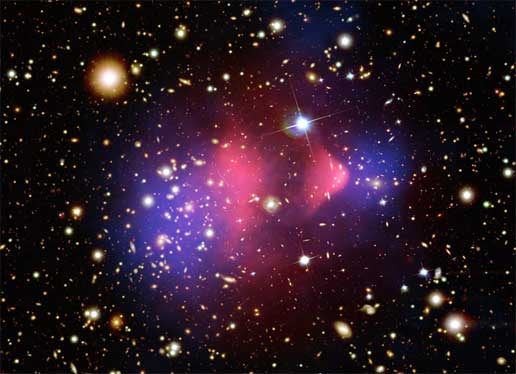
\includegraphics[width=0.8\textwidth]{figures/DMOverview/Bullet_cluster.jpg}
	\caption[An image of the Bullet Cluster highlighting the distribution of mass within the two colliding clusters.]{An image of the Bullet Cluster highlighting the distribution of mass within the two colliding clusters. The pink region indicate where the majority of the baryonic matter is situated formed from X-ray analysis. The blue regions are produced from gravitational micro-lensing measurements highlighting where the total mass of colliding clusters is located \cite{chandra}.}
	\label{fig:DMOverview/BulletComp}
\end{figure}
%MPhil thesis
%Hubble's observations on the Bullet Cluster (1E 0657-56) provides evidence towards the existence of dark matter through gravitational lensing. The Bullet Cluster consists of two clusters of galaxies which have collided and are now moving away from each other. A composite image of the cluster can be seen in figure \ref{fig:BulletComp}. The colouring in the image indicates the distribution of mass within the colliding clusters. The blue regions highlight where most of the mass is and the pink region illustrating where the baryonic matter is situated, predominately gas and dust. Analysis of X-ray studies found that as the two clusters passed through each other the baryonic matter interacted and `clumped' to produce X-rays. Whereas gravitational lensing measurements indicated that the majority of the non-luminous portion of mass continued without disruption. The X-ray peaks of the colliding clusters were compared with the lensing mass peaks of the clusters and an offset was found \cite{Clowe_2004}. The offset found between the X-ray peaks and lensing mass peaks is considered as strong evidence towards the presence of dark matter within the two colliding clusters. Modified theories of Newtonian dynamics were also applied to explain the Bullet Cluster formation. They could not explain this effect fully and the dark matter component in the applied regime was equal to the baryonic mass of the system \cite{Clowe_2004}. Thus the existence of dark matter still holds true. This strengthens the importance of the Bullet Cluster observations as evidence towards the existence of dark matter.

%ChatGPT response
%\section{The Bullet Cluster as Direct Evidence for Dark Matter}
%Observations of the Bullet Cluster , particularly those made by the Hubble Space Telescope and the Chandra X-ray Observatory, provide some of the most compelling empirical evidence for the existence of dark matter through the phenomenon of gravitational lensing.

%The Bullet Cluster comprises two galaxy clusters that have undergone a high-velocity collision and are now moving apart. A composite image of the system is shown in Figure~\ref{fig:BulletComp}, where color overlays represent the distribution of both luminous and total mass components. The blue regions in the image correspond to the total mass distribution derived from gravitational lensing measurements, while the pink regions represent the hot, X-ray-emitting gas that contains the majority of the baryonic (ordinary) matter, such as gas and dust.

%X-ray observations reveal that, as the two clusters passed through one another, their gaseous components interacted strongly—colliding, slowing down, and heating up, thus producing intense X-ray emissions. In contrast, gravitational lensing analysis demonstrated that the bulk of the total mass—dominated by a non-luminous component—continued on its trajectory relatively unimpeded, showing minimal interaction \cite{Clowe_2004}.

%This resulted in a measurable spatial offset between the peaks of the X-ray emissions (tracing baryonic matter) and the peaks of the lensing mass distribution (tracing total mass), as illustrated in Figure~\ref{fig:BulletComp}. The existence of this offset indicates that the dominant mass component is not collisional like gas, but rather behaves as collisionless matter—one of the key predicted properties of dark matter.

%Alternative gravitational models, such as Modified Newtonian Dynamics (MOND), have been proposed to explain such observations without invoking dark matter. However, these theories struggle to account for the Bullet Cluster’s observed separation of mass and baryonic matter. In order to reconcile the data, even MOND-like frameworks require a dark matter component with a mass comparable to the visible baryonic matter \cite{Clowe_2004}. 

%Thus, the Bullet Cluster serves as a natural laboratory in which dark matter can be isolated and studied independently of baryonic matter. Its observations strongly reinforce the dark matter paradigm and challenge alternative gravity-based explanations.



\section{The Cosmic Microwave Background}\label{sec:DMOverview/CMB}

\subsection{$\Lambda$CDM model}\label{sec:DMOverview/LambdaCDM}

\section{Avoiding dark matter}\label{sec:DMOverview/AvoidDM}

\subsection{Modification of Newtonian dynamics}\label{sec:DMOverview/MOND}

\subsection{MACHOs}\label{sec:DMOverview/MACHOs}

\section{Possible candidates for dark matter}\label{sec:DMOverview/Candidates4DM}

\subsubsection{WIMPs}\label{sec:DMOverview/WIMPs}

\subsection{Sterile neutrinos}\label{sec:DMOverview/Neutrinos}

\subsection{Axions}\label{sec:DMOverview/Axions}

\section{Searching for dark matter}\label{sec:DMOverview/DetectionOfDM}

\subsection{Indirect detection of dark matter}\label{sec:DMOverview/IndirectDM}

\subsection{Dark matter production at colliders}\label{sec:DMOverview/DMProdColliders}

\subsection{Direct detection of dark matter}\label{sec:DMOverview/DirectDetection}

\section{Current status for dark matter searches}\label{sec:DMOverview/DMCurrentStatus}